\chapter{Appendix. Large-scale urban traffic microsimulations}
\chaptermark{Appendix. Large-scale urban traffic microsimulations}
\label{ch:appendix_getting_real}

\graphicspath{{chapters/appendix_ETRCO2H/figures}}

\section{Statistical information}
\label{sec:appendix}


\begin{figure*}[ht!]
    \centering
    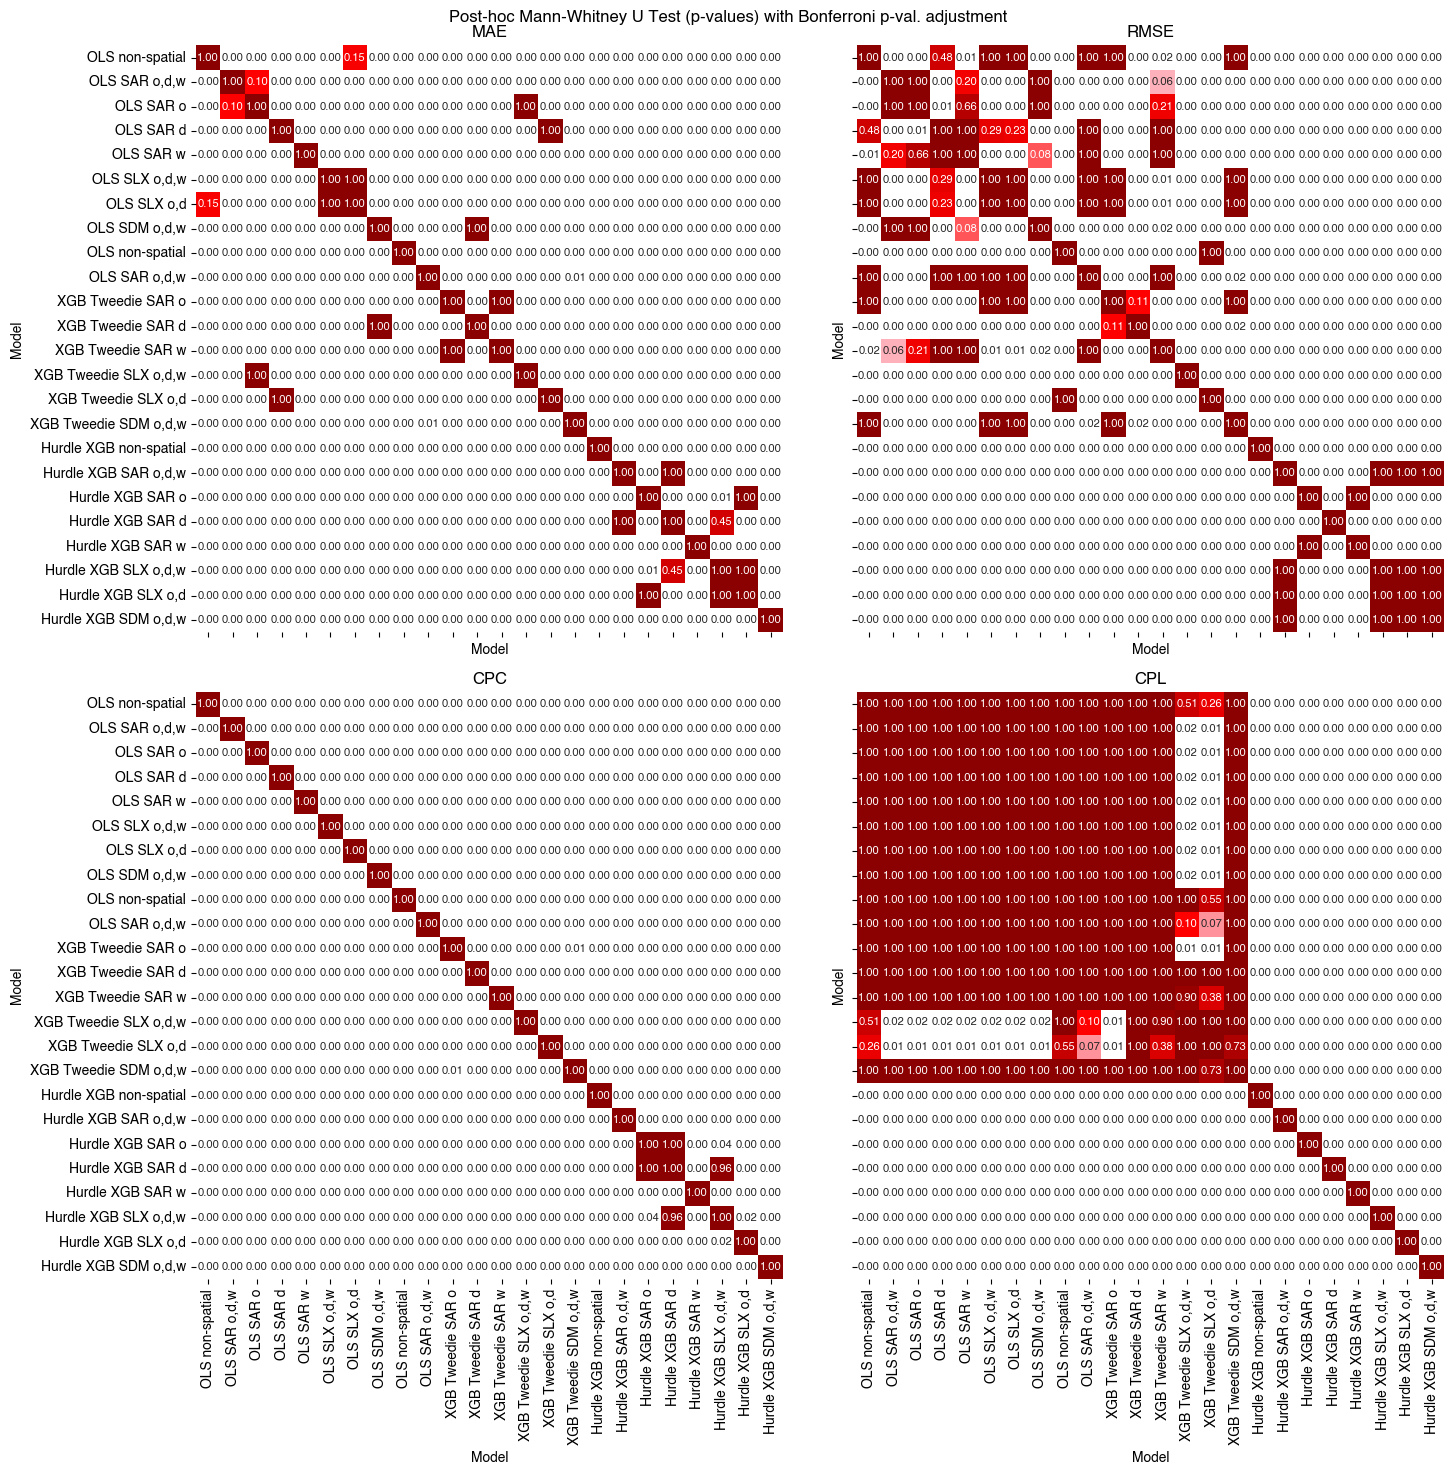
\includegraphics[width=1\textwidth]{fig_MWU_results_models_Bonf_n1000_r.png}
    \caption{Pairwise comparison between the goodness-of-fit metrics for all considered models. We show $p$-values  resulting from a Mann-Whitney-U non-parametric test \citep{Mann1947}, after applying the Bonferroni method for $p$-value correction for multiple comparisons. In most cases, the different models and spatial interaction specifications exhibit statistically significant differences ($p<0.05$). Only CPL shows consistent acceptance of the null hypothesis ($p>0.05$) (i.e. the results of the models are statistically equivalent) for the different specifications of the one-part OLS and XGBoost Tweedie models.}
    \label{fig:MWU_test_2x2_pvalues}
\end{figure*}

\begin{figure*}[ht!]
    \centering
    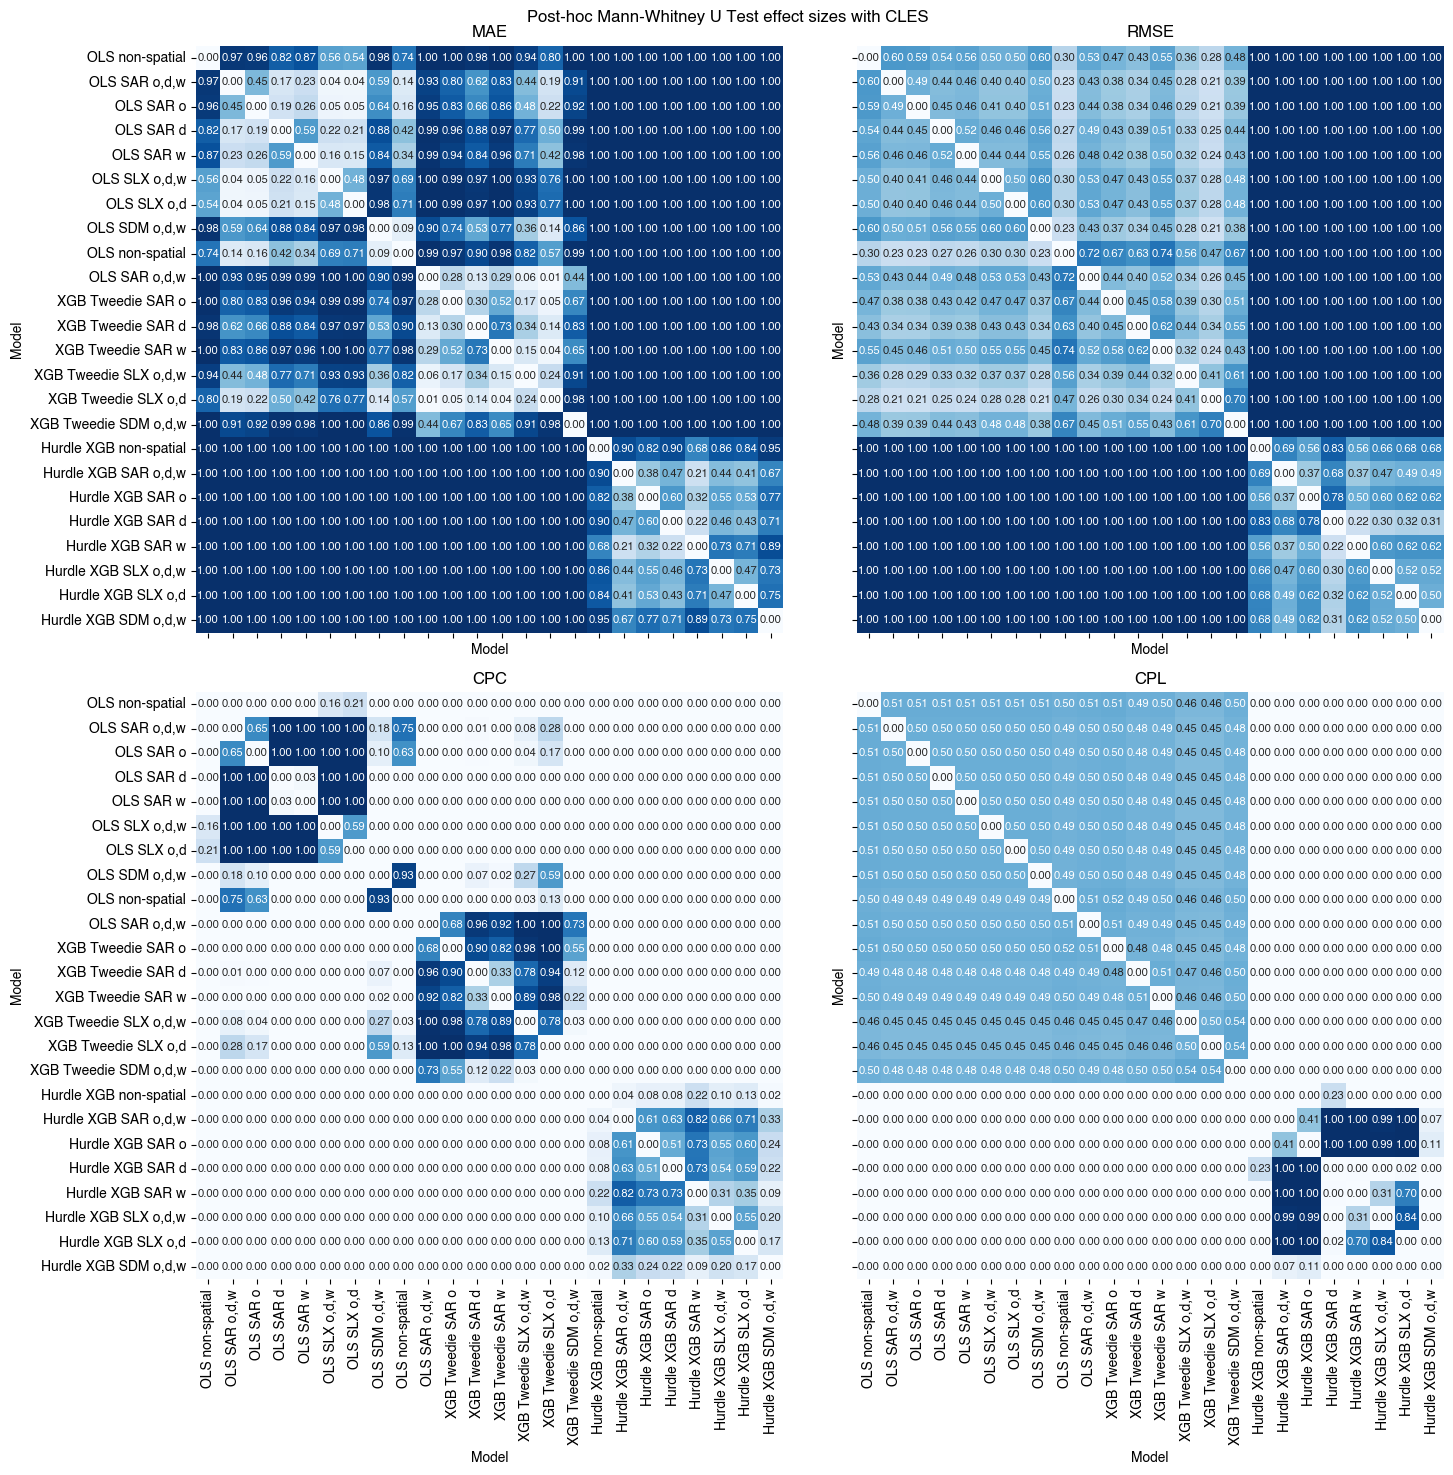
\includegraphics[width=1\textwidth]{fig_MWU_results_Bonf_effect_size_CLES_n1000_r.png}
    \caption{Common Language Effect Size (CLES) \citep{Vargha2000AWong} from the pairwise comparison between the goodness-of-fit metrics for all considered models resulting from a Mann-Whitney-U non-parametric test \citep{Mann1947}.}
    \label{fig:MWU_test_2x2_effectSize}
\end{figure*}

% % \usepackage{rotating}
% \usepackage{tabularray}
\begin{table*}[ht!]
\centering
\caption{Results of Ordinary Least Squares models.}
\label{tab:append_results_ols_SHP}
\resizebox{\linewidth}{!}{%
\begin{tblr}{
rowsep=1pt,
colsep=1pt,
  cell{1}{3} = {c=31}{c},
  cell{2}{3} = {c=3}{c},
  cell{2}{6} = {c},
  cell{2}{7} = {c=15}{c},
  cell{2}{22} = {c},
  cell{2}{23} = {c=7}{c},
  cell{2}{30} = {c},
  cell{2}{31} = {c=3}{c},
  cell{3}{2} = {r},
  cell{3}{5} = {c},
  cell{3}{6} = {c},
  cell{3}{7} = {c=3}{c},
  cell{3}{10} = {c},
  cell{3}{11} = {c=3}{c},
  cell{3}{14} = {c},
  cell{3}{15} = {c=3}{c},
  cell{3}{18} = {c},
  cell{3}{19} = {c=3}{c},
  cell{3}{22} = {c},
  cell{3}{23} = {c=3}{c},
  cell{3}{26} = {c},
  cell{3}{27} = {c=3}{c},
  cell{3}{30} = {c},
  cell{3}{31} = {c=3}{c},
  cell{5}{3} = {r},
  cell{5}{7} = {r},
  cell{5}{11} = {r},
  cell{5}{15} = {r},
  cell{5}{19} = {r},
  cell{5}{23} = {r},
  cell{5}{27} = {r},
  cell{5}{31} = {r},
  cell{6}{1} = {r=23}{},
  cell{6}{3} = {r},
  cell{6}{7} = {r},
  cell{6}{11} = {r},
  cell{6}{15} = {r},
  cell{6}{19} = {r},
  cell{6}{23} = {r},
  cell{6}{27} = {r},
  cell{6}{31} = {r},
  cell{7}{3} = {r},
  cell{7}{7} = {r},
  cell{7}{11} = {r},
  cell{7}{15} = {r},
  cell{7}{19} = {r},
  cell{7}{23} = {r},
  cell{7}{27} = {r},
  cell{7}{31} = {r},
  cell{8}{3} = {r},
  cell{8}{7} = {r},
  cell{8}{11} = {r},
  cell{8}{15} = {r},
  cell{8}{19} = {r},
  cell{8}{23} = {r},
  cell{8}{27} = {r},
  cell{8}{31} = {r},
  cell{9}{3} = {r},
  cell{9}{7} = {r},
  cell{9}{11} = {r},
  cell{9}{15} = {r},
  cell{9}{19} = {r},
  cell{9}{23} = {r},
  cell{9}{27} = {r},
  cell{9}{31} = {r},
  cell{10}{3} = {r},
  cell{10}{7} = {r},
  cell{10}{11} = {r},
  cell{10}{15} = {r},
  cell{10}{19} = {r},
  cell{10}{23} = {r},
  cell{10}{27} = {r},
  cell{10}{31} = {r},
  cell{11}{3} = {r},
  cell{11}{7} = {r},
  cell{11}{11} = {r},
  cell{11}{15} = {r},
  cell{11}{19} = {r},
  cell{11}{23} = {r},
  cell{11}{27} = {r},
  cell{11}{31} = {r},
  cell{12}{3} = {r},
  cell{12}{7} = {r},
  cell{12}{11} = {r},
  cell{12}{15} = {r},
  cell{12}{19} = {r},
  cell{12}{23} = {r},
  cell{12}{27} = {r},
  cell{12}{31} = {r},
  cell{13}{3} = {r},
  cell{13}{7} = {r},
  cell{13}{11} = {r},
  cell{13}{15} = {r},
  cell{13}{19} = {r},
  cell{13}{23} = {r},
  cell{13}{27} = {r},
  cell{13}{31} = {r},
  cell{14}{3} = {r},
  cell{14}{7} = {r},
  cell{14}{11} = {r},
  cell{14}{15} = {r},
  cell{14}{19} = {r},
  cell{14}{23} = {r},
  cell{14}{27} = {r},
  cell{14}{31} = {r},
  cell{15}{3} = {r},
  cell{15}{7} = {r},
  cell{15}{11} = {r},
  cell{15}{15} = {r},
  cell{15}{19} = {r},
  cell{15}{23} = {r},
  cell{15}{27} = {r},
  cell{15}{31} = {r},
  cell{16}{3} = {r},
  cell{16}{7} = {r},
  cell{16}{11} = {r},
  cell{16}{15} = {r},
  cell{16}{19} = {r},
  cell{16}{23} = {r},
  cell{16}{27} = {r},
  cell{16}{31} = {r},
  cell{17}{3} = {r},
  cell{17}{7} = {r},
  cell{17}{11} = {r},
  cell{17}{15} = {r},
  cell{17}{19} = {r},
  cell{17}{23} = {r},
  cell{17}{27} = {r},
  cell{17}{31} = {r},
  cell{18}{3} = {r},
  cell{18}{7} = {r},
  cell{18}{11} = {r},
  cell{18}{15} = {r},
  cell{18}{19} = {r},
  cell{18}{23} = {r},
  cell{18}{27} = {r},
  cell{18}{31} = {r},
  cell{19}{3} = {r},
  cell{19}{7} = {r},
  cell{19}{11} = {r},
  cell{19}{15} = {r},
  cell{19}{19} = {r},
  cell{19}{23} = {r},
  cell{19}{27} = {r},
  cell{19}{31} = {r},
  cell{20}{3} = {r},
  cell{20}{7} = {r},
  cell{20}{11} = {r},
  cell{20}{15} = {r},
  cell{20}{19} = {r},
  cell{20}{23} = {r},
  cell{20}{27} = {r},
  cell{20}{31} = {r},
  cell{21}{3} = {r},
  cell{21}{7} = {r},
  cell{21}{11} = {r},
  cell{21}{15} = {r},
  cell{21}{19} = {r},
  cell{21}{23} = {r},
  cell{21}{27} = {r},
  cell{21}{31} = {r},
  cell{22}{3} = {r},
  cell{22}{7} = {r},
  cell{22}{11} = {r},
  cell{22}{15} = {r},
  cell{22}{19} = {r},
  cell{22}{23} = {r},
  cell{22}{27} = {r},
  cell{22}{31} = {r},
  cell{23}{3} = {r},
  cell{23}{7} = {r},
  cell{23}{11} = {r},
  cell{23}{15} = {r},
  cell{23}{19} = {r},
  cell{23}{23} = {r},
  cell{23}{27} = {r},
  cell{23}{31} = {r},
  cell{24}{3} = {r},
  cell{24}{7} = {r},
  cell{24}{11} = {r},
  cell{24}{15} = {r},
  cell{24}{19} = {r},
  cell{24}{23} = {r},
  cell{24}{27} = {r},
  cell{24}{31} = {r},
  cell{25}{3} = {r},
  cell{25}{7} = {r},
  cell{25}{11} = {r},
  cell{25}{15} = {r},
  cell{25}{19} = {r},
  cell{25}{23} = {r},
  cell{25}{27} = {r},
  cell{25}{31} = {r},
  cell{26}{3} = {r},
  cell{26}{7} = {r},
  cell{26}{11} = {r},
  cell{26}{15} = {r},
  cell{26}{19} = {r},
  cell{26}{23} = {r},
  cell{26}{27} = {r},
  cell{26}{31} = {r},
  cell{27}{3} = {r},
  cell{27}{7} = {r},
  cell{27}{11} = {r},
  cell{27}{15} = {r},
  cell{27}{19} = {r},
  cell{27}{23} = {r},
  cell{27}{27} = {r},
  cell{27}{31} = {r},
  cell{28}{3} = {r},
  cell{28}{7} = {r},
  cell{28}{11} = {r},
  cell{28}{15} = {r},
  cell{28}{19} = {r},
  cell{28}{23} = {r},
  cell{28}{27} = {r},
  cell{28}{31} = {r},
  cell{29}{1} = {r=23}{},
  cell{29}{23} = {r},
  cell{29}{27} = {r},
  cell{29}{31} = {r},
  cell{30}{23} = {r},
  cell{30}{27} = {r},
  cell{30}{31} = {r},
  cell{31}{23} = {r},
  cell{31}{27} = {r},
  cell{31}{31} = {r},
  cell{32}{23} = {r},
  cell{32}{27} = {r},
  cell{32}{31} = {r},
  cell{33}{23} = {r},
  cell{33}{27} = {r},
  cell{33}{31} = {r},
  cell{34}{23} = {r},
  cell{34}{27} = {r},
  cell{34}{31} = {r},
  cell{35}{23} = {r},
  cell{35}{27} = {r},
  cell{35}{31} = {r},
  cell{36}{23} = {r},
  cell{36}{27} = {r},
  cell{36}{31} = {r},
  cell{37}{23} = {r},
  cell{37}{27} = {r},
  cell{37}{31} = {r},
  cell{38}{23} = {r},
  cell{38}{27} = {r},
  cell{38}{31} = {r},
  cell{39}{23} = {r},
  cell{39}{27} = {r},
  cell{39}{31} = {r},
  cell{40}{23} = {r},
  cell{40}{27} = {r},
  cell{40}{31} = {r},
  cell{41}{23} = {r},
  cell{41}{27} = {r},
  cell{41}{31} = {r},
  cell{42}{23} = {r},
  cell{42}{27} = {r},
  cell{42}{31} = {r},
  cell{43}{23} = {r},
  cell{43}{27} = {r},
  cell{43}{31} = {r},
  cell{44}{23} = {r},
  cell{44}{27} = {r},
  cell{44}{31} = {r},
  cell{45}{23} = {r},
  cell{45}{27} = {r},
  cell{45}{31} = {r},
  cell{46}{23} = {r},
  cell{46}{27} = {r},
  cell{46}{31} = {r},
  cell{47}{23} = {r},
  cell{47}{27} = {r},
  cell{47}{31} = {r},
  cell{48}{23} = {r},
  cell{48}{27} = {r},
  cell{48}{31} = {r},
  cell{49}{23} = {r},
  cell{49}{27} = {r},
  cell{49}{31} = {r},
  cell{50}{23} = {r},
  cell{50}{27} = {r},
  cell{50}{31} = {r},
  cell{51}{23} = {r},
  cell{51}{31} = {r},
  cell{52}{1} = {r=3}{},
  cell{52}{7} = {r},
  cell{52}{11} = {r},
  cell{52}{31} = {r},
  cell{53}{7} = {r},
  cell{53}{15} = {r},
  cell{53}{31} = {r},
  cell{54}{7} = {r},
  cell{54}{19} = {r},
  cell{54}{31} = {r},
  cell{55}{2} = {r},
  cell{55}{3} = {c=3}{c},
  cell{55}{6} = {c},
  cell{55}{7} = {c=3}{c},
  cell{55}{10} = {c},
  cell{55}{11} = {c=3}{c},
  cell{55}{14} = {c},
  cell{55}{15} = {c=3}{c},
  cell{55}{18} = {c},
  cell{55}{19} = {c=3}{c},
  cell{55}{22} = {c},
  cell{55}{23} = {c=3}{c},
  cell{55}{26} = {c},
  cell{55}{27} = {c=3}{c},
  cell{55}{30} = {c},
  cell{55}{31} = {c=3}{c},
  cell{56}{2} = {r},
  cell{56}{3} = {c=3}{c},
  cell{56}{6} = {c},
  cell{56}{7} = {c=3}{c},
  cell{56}{10} = {c},
  cell{56}{11} = {c=3}{c},
  cell{56}{14} = {c},
  cell{56}{15} = {c=3}{c},
  cell{56}{18} = {c},
  cell{56}{19} = {c=3}{c},
  cell{56}{22} = {c},
  cell{56}{23} = {c=3}{c},
  cell{56}{26} = {c},
  cell{56}{27} = {c=3}{c},
  cell{56}{30} = {c},
  cell{56}{31} = {c=3}{c},
  cell{57}{2} = {r},
  cell{57}{3} = {c=3}{c},
  cell{57}{6} = {c},
  cell{57}{7} = {c=3}{c},
  cell{57}{10} = {c},
  cell{57}{11} = {c=3}{c},
  cell{57}{14} = {c},
  cell{57}{15} = {c=3}{c},
  cell{57}{18} = {c},
  cell{57}{19} = {c=3}{c},
  cell{57}{22} = {c},
  cell{57}{23} = {c=3}{c},
  cell{57}{26} = {c},
  cell{57}{27} = {c=3}{c},
  cell{57}{30} = {c},
  cell{57}{31} = {c=3}{c},
  cell{58}{2} = {r},
  cell{58}{3} = {c=3}{c},
  cell{58}{6} = {c},
  cell{58}{7} = {c=3}{c},
  cell{58}{10} = {c},
  cell{58}{11} = {c=3}{c},
  cell{58}{14} = {c},
  cell{58}{15} = {c=3}{c},
  cell{58}{18} = {c},
  cell{58}{19} = {c=3}{c},
  cell{58}{22} = {c},
  cell{58}{23} = {c=3}{c},
  cell{58}{26} = {c},
  cell{58}{27} = {c=3}{c},
  cell{58}{30} = {c},
  cell{58}{31} = {c=3}{c},
  cell{59}{2} = {r},
  cell{59}{3} = {c=3}{c},
  cell{59}{6} = {c},
  cell{59}{7} = {c=3}{c},
  cell{59}{10} = {c},
  cell{59}{11} = {c=3}{c},
  cell{59}{14} = {c},
  cell{59}{15} = {c=3}{c},
  cell{59}{18} = {c},
  cell{59}{19} = {c=3}{c},
  cell{59}{22} = {c},
  cell{59}{23} = {c=3}{c},
  cell{59}{26} = {c},
  cell{59}{27} = {c=3}{c},
  cell{59}{30} = {c},
  cell{59}{31} = {c=3}{c},
  cell{60}{2} = {r},
  cell{60}{3} = {c=3}{c},
  cell{60}{6} = {c},
  cell{60}{7} = {c=3}{c},
  cell{60}{10} = {c},
  cell{60}{11} = {c=3}{c},
  cell{60}{14} = {c},
  cell{60}{15} = {c=3}{c},
  cell{60}{18} = {c},
  cell{60}{19} = {c=3}{c},
  cell{60}{22} = {c},
  cell{60}{23} = {c=3}{c},
  cell{60}{26} = {c},
  cell{60}{27} = {c=3}{c},
  cell{60}{30} = {c},
  cell{60}{31} = {c=3}{c},
  hline{1,61} = {-}{0.08em},
  hline{2} = {3-33}{},
  hline{3} = {3-5,7-21,23-29,31-33}{},
  hline{4} = {7-9,11-13,15-17,19-21,23-25,27-29,31-33}{},
  hline{5} = {1-5,7-33}{},
  hline{29,52} = {1}{},
  hline{55} = {-}{},
}
                                                                              & \textbf{model}                                          & \textbf{OLS}      &     &                &  &                         &     &                &  &                     &     &                &  &                     &     &                &  &                     &     &                &  &                         &     &                &  &                       &     &                &  &                         &     &                \\
                                                                              & \textbf{spatial interaction}                            & \textbf{baseline} &     &                &  & \textbf{SAR}            &     &                &  &                     &     &                &  &                     &     &                &  &                     &     &                &  & \textbf{SLX}            &     &                &  &                       &     &                &  & \textbf{SDM}            &     &                \\
                                                                              & \textit{\textbf{filtering}}                             &                   &     &                &  & \textit{\textbf{o,d,w}} &     &                &  & \textit{\textbf{o}} &     &                &  & \textit{\textbf{d}} &     &                &  & \textit{\textbf{w}} &     &                &  & \textit{\textbf{o,d,w}} &     &                &  & \textit{\textbf{o,d}} &     &                &  & \textit{\textbf{o,d,w}} &     &                \\
                                                                              &                                                         & \textit{coeff}    &     & \textit{p-val} &  & \textit{coeff}          &     & \textit{p-val} &  & \textit{coeff}      &     & \textit{p-val} &  & \textit{coeff}      &     & \textit{p-val} &  & \textit{coeff}      &     & \textit{p-val} &  & \textit{coeff}          &     & \textit{p-val} &  & \textit{coeff}        &     & \textit{p-val} &  & \textit{coeff}          &     & \textit{p-val} \\
                                                                              & \textit{constant}                                       & 22.361            & *** & 0.000          &  & 5.866                   & *** & 0.000          &  & 6.922               & *** & 0.000          &  & 11.614              & *** & 0.000          &  & 12.172              & *** & 0.000          &  & 33.047                  & *** & 0.000          &  & 34.898                & *** & 0.000          &  & 9.604                   & *** & 0.000          \\
\begin{sideways}\textbf{Independent variables X}\end{sideways}                & \textit{log\_quickest\_traveltime}                      & -2.692            & *** & 0.000          &  & -1.530                  & *** & 0.000          &  & -1.618              & *** & 0.000          &  & -1.937              & *** & 0.000          &  & -1.897              & *** & 0.000          &  & -3.254                  & *** & 0.000          &  & -2.962                & *** & 0.000          &  & -2.708                  & *** & 0.000          \\
                                                                              & \textit{log\_quickest\_route\_centrality\_mean}         & 0.028             &     & 0.413          &  & 0.228                   & *** & 0.000          &  & 0.194               & *** & 0.000          &  & 0.145               & *** & 0.000          &  & 0.285               & *** & 0.000          &  & -0.207                  & **  & 0.005          &  & -0.141                & *** & 0.000          &  & -0.025                  &     & 0.690          \\
                                                                              & \textit{log\_quickest\_route\_centrality\_max}          & -0.677            & *** & 0.000          &  & -0.222                  & *** & 0.000          &  & -0.230              & *** & 0.000          &  & -0.389              & *** & 0.000          &  & -0.495              & *** & 0.000          &  & -0.224                  & *** & 0.000          &  & -0.530                & *** & 0.000          &  & -0.173                  & **  & 0.001          \\
                                                                              & \textit{log\_quickest\_route\_centrality\_min}          & -0.256            & *** & 0.000          &  & -0.175                  & *** & 0.000          &  & -0.177              & *** & 0.000          &  & -0.201              & *** & 0.000          &  & -0.227              & *** & 0.000          &  & -0.214                  & *** & 0.000          &  & -0.172                & *** & 0.000          &  & -0.140                  & *** & 0.000          \\
                                                                              & \textit{log\_o\_pop\_dens\_inh\_per\_km2}               & -0.341            & *** & 0.000          &  & -0.176                  & *** & 0.000          &  & -0.193              & *** & 0.000          &  & -0.231              & *** & 0.000          &  & -0.210              & *** & 0.000          &  & -0.100                  & *** & 0.000          &  & -0.167                & *** & 0.000          &  & 0.002                   &     & 0.780          \\
                                                                              & \textit{log\_o\_area\_const\_sum\_V}                    & 0.474             & *** & 0.000          &  & 0.400                   & *** & 0.000          &  & 0.398               & *** & 0.000          &  & 0.446               & *** & 0.000          &  & 0.438               & *** & 0.000          &  & 0.461                   & *** & 0.000          &  & 0.507                 & *** & 0.000          &  & 0.484                   & *** & 0.000          \\
                                                                              & \textit{log\_o\_area\_const\_sum\_C}                    & 0.033             & *** & 0.000          &  & -0.034                  & *** & 0.000          &  & -0.027              & *** & 0.000          &  & -0.020              & **  & 0.004          &  & -0.008              &     & 0.256          &  & 0.023                   & **  & 0.006          &  & 0.023                 & **  & 0.005          &  & -0.016                  & *   & 0.019          \\
                                                                              & \textit{log\_o\_area\_const\_sum\_O}                    & -0.021            & *** & 0.000          &  & -0.027                  & *** & 0.000          &  & -0.027              & *** & 0.000          &  & -0.021              & *** & 0.000          &  & -0.029              & *** & 0.000          &  & -0.019                  & *** & 0.000          &  & -0.020                & *** & 0.000          &  & -0.013                  & *** & 0.000          \\
                                                                              & \textit{log\_o\_area\_const\_sum\_E}                    & -0.011            & **  & 0.001          &  & -0.006                  & *   & 0.044          &  & -0.003              &     & 0.256          &  & -0.012              & *** & 0.000          &  & -0.019              & *** & 0.000          &  & -0.008                  & *   & 0.031          &  & -0.007                & *   & 0.045          &  & -0.005                  &     & 0.083          \\
                                                                              & \textit{log\_o\_area\_const\_sum\_A}                    & 0.103             & *** & 0.000          &  & 0.133                   & *** & 0.000          &  & 0.136               & *** & 0.000          &  & 0.118               & *** & 0.000          &  & 0.101               & *** & 0.000          &  & 0.085                   & *** & 0.000          &  & 0.096                 & *** & 0.000          &  & 0.080                   & *** & 0.000          \\
                                                                              & \textit{log\_o\_ratio\_workers}                         & 0.408             & *** & 0.000          &  & 0.350                   & *** & 0.000          &  & 0.364               & *** & 0.000          &  & 0.375               & *** & 0.000          &  & 0.310               & *** & 0.000          &  & 0.729                   & *** & 0.000          &  & 0.715                 & *** & 0.000          &  & 0.793                   & *** & 0.000          \\
                                                                              & \textit{log\_o\_len\_\_non\_motorways\_per\_km2}        & -0.036            & *** & 0.000          &  & -0.033                  & *** & 0.000          &  & -0.032              & *** & 0.000          &  & -0.035              & *** & 0.000          &  & -0.038              & *** & 0.000          &  & -0.003                  &     & 0.389          &  & -0.003                &     & 0.444          &  & -0.001                  &     & 0.723          \\
                                                                              & \textit{log\_o\_ratio\_GHSL\_built\_6to15m}             & 3.333             & *** & 0.000          &  & 2.172                   & *** & 0.000          &  & 2.179               & *** & 0.000          &  & 2.572               & *** & 0.000          &  & 2.984               & *** & 0.000          &  & 1.766                   & *** & 0.000          &  & 1.673                 & *** & 0.000          &  & 1.466                   & *** & 0.000          \\
                                                                              & \textit{log\_d\_pop\_dens\_inh\_per\_km2}               & -0.355            & *** & 0.000          &  & -0.227                  & *** & 0.000          &  & -0.233              & *** & 0.000          &  & -0.275              & *** & 0.000          &  & -0.282              & *** & 0.000          &  & -0.151                  & *** & 0.000          &  & -0.182                & *** & 0.000          &  & -0.060                  & *** & 0.000          \\
                                                                              & \textit{log\_d\_area\_const\_sum\_V}                    & 0.464             & *** & 0.000          &  & 0.152                   & *** & 0.000          &  & 0.183               & *** & 0.000          &  & 0.246               & *** & 0.000          &  & 0.232               & *** & 0.000          &  & 0.471                   & *** & 0.000          &  & 0.493                 & *** & 0.000          &  & 0.086                   & *** & 0.000          \\
                                                                              & \textit{log\_d\_area\_const\_sum\_C}                    & 0.046             & *** & 0.000          &  & 0.002                   &     & 0.745          &  & 0.005               &     & 0.441          &  & 0.017               & *   & 0.019          &  & 0.020               & **  & 0.004          &  & 0.024                   & **  & 0.003          &  & 0.022                 & **  & 0.008          &  & 0.005                   &     & 0.470          \\
                                                                              & \textit{log\_d\_area\_const\_sum\_O}                    & -0.043            & *** & 0.000          &  & -0.022                  & *** & 0.000          &  & -0.021              & *** & 0.000          &  & -0.039              & *** & 0.000          &  & -0.029              & *** & 0.000          &  & -0.039                  & *** & 0.000          &  & -0.042                & *** & 0.000          &  & -0.011                  & *** & 0.000          \\
                                                                              & \textit{log\_d\_area\_const\_sum\_E}                    & 0.005             &     & 0.122          &  & -0.008                  & **  & 0.006          &  & -0.009              & **  & 0.002          &  & 0.006               &     & 0.055          &  & -0.006              & *   & 0.043          &  & 0.015                   & *** & 0.000          &  & 0.013                 & *** & 0.000          &  & 0.001                   &     & 0.819          \\
                                                                              & \textit{log\_d\_area\_const\_sum\_A}                    & 0.130             & *** & 0.000          &  & 0.058                   & *** & 0.000          &  & 0.060               & *** & 0.000          &  & 0.107               & *** & 0.000          &  & 0.071               & *** & 0.000          &  & 0.133                   & *** & 0.000          &  & 0.139                 & *** & 0.000          &  & 0.035                   & *** & 0.000          \\
                                                                              & \textit{log\_d\_ratio\_workers}                         & 0.592             & *** & 0.000          &  & -0.001                  &     & 0.964          &  & 0.037               &     & 0.100          &  & 0.284               & *** & 0.000          &  & 0.118               & *** & 0.000          &  & 0.909                   & *** & 0.000          &  & 0.893                 & *** & 0.000          &  & 0.204                   & *** & 0.000          \\
                                                                              & \textit{log\_d\_len\_\_non\_motorways\_per\_km2}        & -0.041            & *** & 0.000          &  & -0.019                  & *** & 0.000          &  & -0.019              & *** & 0.000          &  & -0.030              & *** & 0.000          &  & -0.027              & *** & 0.000          &  & -0.015                  & *** & 0.000          &  & -0.013                & *** & 0.000          &  & 0.000                   &     & 0.949          \\
                                                                              & \textit{log\_d\_ratio\_GHSL\_built\_6to15m}             & 3.292             & *** & 0.000          &  & 1.304                   & *** & 0.000          &  & 1.441               & *** & 0.000          &  & 1.972               & *** & 0.000          &  & 2.050               & *** & 0.000          &  & 1.512                   & *** & 0.000          &  & 1.504                 & *** & 0.000          &  & 0.285                   & **  & 0.004          \\
                                                                              & \textit{log\_graph\_degree}                             & -0.778            & *** & 0.000          &  & 0.807                   & *** & 0.000          &  & 0.701               & *** & 0.000          &  & 0.294               & *** & 0.000          &  & 0.174               & *** & 0.000          &  & -3.374                  & *** & 0.000          &  & -0.587                & *** & 0.000          &  & -0.384                  & **  & 0.002          \\
\begin{sideways}\textbf{spatial lag of independent variables X}\end{sideways} & \textit{log\_Wq\_R\_quickest\_traveltime}               &                   &     &                &  &                         &     &                &  &                     &     &                &  &                     &     &                &  &                     &     &                &  & 0.805                   & *** & 0.000          &  &                       &     &                &  & 2.273                   & *** & 0.000          \\
                                                                              & \textit{log\_Wq\_R\_quickest\_route\_centrality\_mean}  &                   &     &                &  &                         &     &                &  &                     &     &                &  &                     &     &                &  &                     &     &                &  & -0.116                  &     & 0.174          &  &                       &     &                &  & -0.109                  &     & 0.128          \\
                                                                              & \textit{log\_Wq\_R\_quickest\_route\_centrality\_max}   &                   &     &                &  &                         &     &                &  &                     &     &                &  &                     &     &                &  &                     &     &                &  & -0.333                  & *** & 0.000          &  &                       &     &                &  & 0.074                   &     & 0.220          \\
                                                                              & \textit{log\_Wq\_R\_quickest\_route\_centrality\_min}   &                   &     &                &  &                         &     &                &  &                     &     &                &  &                     &     &                &  &                     &     &                &  & 0.092                   & *** & 0.000          &  &                       &     &                &  & 0.049                   & **  & 0.003          \\
                                                                              & \textit{log\_Wq\_R\_o\_pop\_dens\_inh\_per\_km2}        &                   &     &                &  &                         &     &                &  &                     &     &                &  &                     &     &                &  &                     &     &                &  & -0.341                  & *** & 0.000          &  & -0.343                & *** & 0.000          &  & -0.125                  & *** & 0.000          \\
                                                                              & \textit{log\_Wq\_R\_o\_area\_const\_sum\_V}             &                   &     &                &  &                         &     &                &  &                     &     &                &  &                     &     &                &  &                     &     &                &  & -0.572                  & *** & 0.000          &  & -0.598                & *** & 0.000          &  & -0.752                  & *** & 0.000          \\
                                                                              & \textit{log\_Wq\_R\_o\_area\_const\_sum\_C}             &                   &     &                &  &                         &     &                &  &                     &     &                &  &                     &     &                &  &                     &     &                &  & 0.045                   & *   & 0.012          &  & 0.066                 & *** & 0.000          &  & -0.038                  & *   & 0.012          \\
                                                                              & \textit{log\_Wq\_R\_o\_area\_const\_sum\_O}             &                   &     &                &  &                         &     &                &  &                     &     &                &  &                     &     &                &  &                     &     &                &  & -0.093                  & *** & 0.000          &  & -0.094                & *** & 0.000          &  & -0.056                  & *** & 0.000          \\
                                                                              & \textit{log\_Wq\_R\_o\_area\_const\_sum\_E}             &                   &     &                &  &                         &     &                &  &                     &     &                &  &                     &     &                &  &                     &     &                &  & -0.058                  & *** & 0.000          &  & -0.063                & *** & 0.000          &  & 0.062                   & *** & 0.000          \\
                                                                              & \textit{log\_Wq\_R\_o\_area\_const\_sum\_A}             &                   &     &                &  &                         &     &                &  &                     &     &                &  &                     &     &                &  &                     &     &                &  & 0.448                   & *** & 0.000          &  & 0.444                 & *** & 0.000          &  & 0.212                   & *** & 0.000          \\
                                                                              & \textit{log\_Wq\_R\_o\_ratio\_workers}                  &                   &     &                &  &                         &     &                &  &                     &     &                &  &                     &     &                &  &                     &     &                &  & 0.049                   &     & 0.114          &  & 0.034                 &     & 0.268          &  & -0.443                  & *** & 0.000          \\
                                                                              & \textit{log\_Wq\_R\_o\_len\_\_non\_motorways\_per\_km2} &                   &     &                &  &                         &     &                &  &                     &     &                &  &                     &     &                &  &                     &     &                &  & -0.148                  & *** & 0.000          &  & -0.186                & *** & 0.000          &  & -0.034                  & *   & 0.013          \\
                                                                              & \textit{log\_Wq\_R\_o\_ratio\_GHSL\_built\_6to15m}      &                   &     &                &  &                         &     &                &  &                     &     &                &  &                     &     &                &  &                     &     &                &  & 2.879                   & *** & 0.000          &  & 3.144                 & *** & 0.000          &  & 0.104                   &     & 0.508          \\
                                                                              & \textit{log\_Wq\_R\_d\_pop\_dens\_inh\_per\_km2}        &                   &     &                &  &                         &     &                &  &                     &     &                &  &                     &     &                &  &                     &     &                &  & -0.356                  & *** & 0.000          &  & -0.391                & *** & 0.000          &  & -0.066                  & *** & 0.000          \\
                                                                              & \textit{log\_Wq\_R\_d\_area\_const\_sum\_V}             &                   &     &                &  &                         &     &                &  &                     &     &                &  &                     &     &                &  &                     &     &                &  & -0.614                  & *** & 0.000          &  & -0.581                & *** & 0.000          &  & -0.216                  & *** & 0.000          \\
                                                                              & \textit{log\_Wq\_R\_d\_area\_const\_sum\_C}             &                   &     &                &  &                         &     &                &  &                     &     &                &  &                     &     &                &  &                     &     &                &  & 0.195                   & *** & 0.000          &  & 0.213                 & *** & 0.000          &  & 0.040                   & **  & 0.008          \\
                                                                              & \textit{log\_Wq\_R\_d\_area\_const\_sum\_O}             &                   &     &                &  &                         &     &                &  &                     &     &                &  &                     &     &                &  &                     &     &                &  & -0.128                  & *** & 0.000          &  & -0.139                & *** & 0.000          &  & -0.032                  & *** & 0.000          \\
                                                                              & \textit{log\_Wq\_R\_d\_area\_const\_sum\_E}             &                   &     &                &  &                         &     &                &  &                     &     &                &  &                     &     &                &  &                     &     &                &  & -0.106                  & *** & 0.000          &  & -0.124                & *** & 0.000          &  & -0.023                  & *   & 0.042          \\
                                                                              & \textit{log\_Wq\_R\_d\_area\_const\_sum\_A}             &                   &     &                &  &                         &     &                &  &                     &     &                &  &                     &     &                &  &                     &     &                &  & 0.393                   & *** & 0.000          &  & 0.394                 & *** & 0.000          &  & 0.126                   & *** & 0.000          \\
                                                                              & \textit{log\_Wq\_R\_d\_ratio\_workers}                  &                   &     &                &  &                         &     &                &  &                     &     &                &  &                     &     &                &  &                     &     &                &  & 0.080                   & *   & 0.010          &  & 0.098                 & **  & 0.002          &  & -0.063                  & *   & 0.016          \\
                                                                              & \textit{log\_Wq\_R\_d\_len\_\_non\_motorways\_per\_km2} &                   &     &                &  &                         &     &                &  &                     &     &                &  &                     &     &                &  &                     &     &                &  & -0.077                  & *** & 0.000          &  & -0.109                & *** & 0.000          &  & -0.013                  &     & 0.328          \\
                                                                              & \textit{log\_Wq\_R\_d\_ratio\_GHSL\_built\_6to15m}      &                   &     &                &  &                         &     &                &  &                     &     &                &  &                     &     &                &  &                     &     &                &  & 3.299                   & *** & 0.000          &  & 3.489                 & *** & 0.000          &  & 0.895                   & *** & 0.000          \\
                                                                              & \textit{log\_Wq\_R\_graph\_degree}                      &                   &     &                &  &                         &     &                &  &                     &     &                &  &                     &     &                &  &                     &     &                &  & 2.504                   & *** & 0.000          &  &                       &     &                &  & 0.418                   & *** & 0.001          \\
\begin{sideways}\textbf{lag of Y}\end{sideways}                               & \textit{Rho (origin)}                                   &                   &     &                &  & 0.481                   & *** & 0.000          &  & 0.585               & *** & 0.000          &  &                     &     &                &  &                     &     &                &  &                         &     &                &  &                       &     &                &  & 0.487                   & *** & 0.000          \\
                                                                              & \textit{Rho (destination)}                              &                   &     &                &  & 0.086                   & *** & 0.000          &  &                     &     &                &  & 0.413               & *** & 0.000          &  &                     &     &                &  &                         &     &                &  &                       &     &                &  & 0.096                   & *** & 0.000          \\
                                                                              & \textit{Rho (origin-destination)}                       &                   &     &                &  & 0.029                   & *** & 0.000          &  &                     &     &                &  &                     &     &                &  & 0.189               & *** & 0.000          &  &                         &     &                &  &                       &     &                &  & 0.029                   & *** & 0.000          \\
                                                                              & \textbf{MAE}                                            & 22.541            &     &                &  & 20.181                  &     &                &  & 20.318              &     &                &  & 21.375              &     &                &  & 21.102              &     &                &  & 22.367                  &     &                &  & 22.416                &     &                &  & 19.9                    &     &                \\
                                                                              & \textbf{RMSE}                                           & 241.448           &     &                &  & 228.177                 &     &                &  & 228.778             &     &                &  & 235.726             &     &                &  & 233.8               &     &                &  & 241.082                 &     &                &  & 241.195               &     &                &  & 227.767                 &     &                \\
                                                                              & \textbf{SVQ (\textgreater{}0.85)}                       & 85.273            &     &                &  & 92.842                  &     &                &  & 92.964              &     &                &  & 91.094              &     &                &  & 90.831              &     &                &  & 86.306                  &     &                &  & 85.625                &     &                &  & 93.442                  &     &                \\
                                                                              & \textbf{CPC}                                            & 0.241             &     &                &  & 0.415                   &     &                &  & 0.41                &     &                &  & 0.328               &     &                &  & 0.353               &     &                &  & 0.253                   &     &                &  & 0.250                 &     &                &  & 0.428                   &     &                \\
                                                                              & \textbf{CPL}                                            & 0.415             &     &                &  & 0.415                   &     &                &  & 0.415               &     &                &  & 0.415               &     &                &  & 0.415               &     &                &  & 0.491                   &     &                &  & 0.415                 &     &                &  & 0.515                   &     &                \\
                                                                              & \textbf{AIC}                                            & 1852306.986       &     &                &  & 1740081.672             &     &                &  & 1742966.317         &     &                &  & 1803937.479         &     &                &  & 1785611.712         &     &                &  & 1847487.473             &     &                &  & 1848547.854           &     &                &  & 1731669.096             &     &                
\end{tblr}
}
\end{table*}
% % \usepackage{rotating}
% \usepackage{tabularray}
\begin{table*}[ht!]
\centering
\caption{Results of XGBoost Tweedie models.}
\label{tab:append_results_xgb_tweedie_SHP}
\resizebox{\linewidth}{!}{%
\begin{tblr}{
  rowsep=0pt,
  column{3} = {c},
  column{4} = {c},
  column{5} = {c},
  column{6} = {c},
  column{7} = {c},
  column{8} = {c},
  column{9} = {c},
  column{10} = {c},
  column{11} = {c},
  column{12} = {c},
  column{13} = {c},
  cell{1}{3} = {c=11}{},
  cell{2}{5} = {c=4}{},
  cell{2}{10} = {c=2}{},
  cell{3}{2} = {r},
  cell{4}{3} = {c=11}{},
  cell{5}{1} = {r=23}{},
  cell{28}{1} = {r=23}{},
  cell{51}{1} = {r=3}{},
  cell{54}{2} = {r},
  cell{55}{2} = {r},
  cell{56}{2} = {r},
  cell{57}{2} = {r},
  cell{58}{2} = {r},
  hline{1,59} = {-}{0.08em},
  hline{2} = {3-13}{},
  hline{3} = {3,5-8,10-11,13}{},
  hline{4-5,54} = {-}{},
  hline{28,51} = {1}{},
}
\begin{sideways}\end{sideways}                                                & \textbf{model}                                          & \textbf{Tweedie XGBoost}   &  &                         &                     &                     &                     &  &                         &                       &  &                         \\
\begin{sideways}\end{sideways}                                                & \textbf{spatial interaction}                            & \textbf{baseline}          &  & \textbf{SAR}            &                     &                     &                     &  & \textbf{SLX}            &                       &  & \textbf{SDM}            \\
\begin{sideways}\end{sideways}                                                & \textit{\textbf{filtering}}                             &                            &  & \textbf{\textit{o,d,w}} & \textbf{\textit{o}} & \textbf{\textit{d}} & \textbf{\textit{w}} &  & \textbf{\textit{o,d,w}} & \textbf{\textit{o,d}} &  & \textbf{\textit{o,d,w}} \\
\begin{sideways}\end{sideways}                                                &                                                         & \textit{mean SHAP~ values} &  &                         &                     &                     &                     &  &                         &                       &  &                         \\
\begin{sideways}\textbf{Independent variables X}\end{sideways}                & \textit{log\_quickest\_traveltime}                      & 2.509                      &  & 1.104                   & 1.129               & 1.878               & 1.824               &  & 1.581                   & 2.742                 &  & 0.990                   \\
                                                                              & \textit{log\_quickest\_route\_centrality\_mean}         & 0.344                      &  & 0.264                   & 0.264               & 0.305               & 0.296               &  & 0.217                   & 0.314                 &  & 0.189                   \\
                                                                              & \textit{log\_quickest\_route\_centrality\_max}          & 0.654                      &  & 0.444                   & 0.450               & 0.571               & 0.488               &  & 0.403                   & 0.564                 &  & 0.302                   \\
                                                                              & \textit{log\_quickest\_route\_centrality\_min}          & 0.343                      &  & 0.274                   & 0.313               & 0.338               & 0.319               &  & 0.278                   & 0.245                 &  & 0.220                   \\
                                                                              & \textit{log\_o\_pop\_dens\_inh\_per\_km2}               & 1.143                      &  & 0.780                   & 0.897               & 1.003               & 0.950               &  & 0.468                   & 0.448                 &  & 0.337                   \\
                                                                              & \textit{log\_o\_area\_const\_sum\_V}                    & 0.333                      &  & 0.348                   & 0.317               & 0.350               & 0.433               &  & 0.296                   & 0.232                 &  & 0.274                   \\
                                                                              & \textit{log\_o\_area\_const\_sum\_C}                    & 0.290                      &  & 0.348                   & 0.331               & 0.342               & 0.326               &  & 0.166                   & 0.192                 &  & 0.171                   \\
                                                                              & \textit{log\_o\_area\_const\_sum\_O}                    & 0.297                      &  & 0.317                   & 0.342               & 0.305               & 0.314               &  & 0.108                   & 0.145                 &  & 0.182                   \\
                                                                              & \textit{log\_o\_area\_const\_sum\_E}                    & 0.323                      &  & 0.367                   & 0.380               & 0.284               & 0.346               &  & 0.168                   & 0.162                 &  & 0.215                   \\
                                                                              & \textit{log\_o\_area\_const\_sum\_A}                    & 0.314                      &  & 0.372                   & 0.364               & 0.295               & 0.313               &  & 0.173                   & 0.162                 &  & 0.194                   \\
                                                                              & \textit{log\_o\_ratio\_workers}                         & 0.253                      &  & 0.301                   & 0.266               & 0.261               & 0.221               &  & 0.148                   & 0.157                 &  & 0.176                   \\
                                                                              & \textit{log\_o\_len\_\_non\_motorways\_per\_km2}        & 0.344                      &  & 0.309                   & 0.346               & 0.296               & 0.308               &  & 0.211                   & 0.165                 &  & 0.178                   \\
                                                                              & \textit{log\_o\_ratio\_GHSL\_built\_6to15m}             & 0.439                      &  & 0.331                   & 0.390               & 0.452               & 0.423               &  & 0.182                   & 0.158                 &  & 0.174                   \\
                                                                              & \textit{log\_d\_pop\_dens\_inh\_per\_km2}               & 0.497                      &  & 0.263                   & 0.324               & 0.382               & 0.354               &  & 0.244                   & 0.250                 &  & 0.176                   \\
                                                                              & \textit{log\_d\_area\_const\_sum\_V}                    & 0.326                      &  & 0.262                   & 0.258               & 0.312               & 0.268               &  & 0.272                   & 0.252                 &  & 0.195                   \\
                                                                              & \textit{log\_d\_area\_const\_sum\_C}                    & 0.521                      &  & 0.300                   & 0.335               & 0.466               & 0.359               &  & 0.332                   & 0.344                 &  & 0.246                   \\
                                                                              & \textit{log\_d\_area\_const\_sum\_O}                    & 0.256                      &  & 0.246                   & 0.243               & 0.255               & 0.228               &  & 0.186                   & 0.167                 &  & 0.162                   \\
                                                                              & \textit{log\_d\_area\_const\_sum\_E}                    & 0.321                      &  & 0.216                   & 0.231               & 0.280               & 0.227               &  & 0.259                   & 0.225                 &  & 0.158                   \\
                                                                              & \textit{log\_d\_area\_const\_sum\_A}                    & 0.234                      &  & 0.190                   & 0.196               & 0.207               & 0.162               &  & 0.130                   & 0.161                 &  & 0.132                   \\
                                                                              & \textit{log\_d\_ratio\_workers}                         & 0.253                      &  & 0.217                   & 0.221               & 0.238               & 0.221               &  & 0.208                   & 0.191                 &  & 0.158                   \\
                                                                              & \textit{log\_d\_len\_\_non\_motorways\_per\_km2}        & 0.281                      &  & 0.210                   & 0.195               & 0.288               & 0.230               &  & 0.204                   & 0.257                 &  & 0.140                   \\
                                                                              & \textit{log\_d\_ratio\_GHSL\_built\_6to15m}             & 0.323                      &  & 0.221                   & 0.223               & 0.264               & 0.234               &  & 0.183                   & 0.203                 &  & 0.143                   \\
                                                                              & \textit{log\_graph\_degree}                             & 0.829                      &  & 0.352                   & 0.365               & 0.634               & 0.648               &  & 0.341                   & 0.851                 &  & 0.189                   \\
\begin{sideways}\textbf{spatial lag of independent variables X}\end{sideways} & \textit{log\_Wq\_R\_quickest\_traveltime}               &                            &  &                         &                     &                     &                     &  & 0.686                   &                       &  & 0.517                   \\
                                                                              & \textit{log\_Wq\_R\_quickest\_route\_centrality\_mean}  &                            &  &                         &                     &                     &                     &  & 0.244                   &                       &  & 0.221                   \\
                                                                              & \textit{log\_Wq\_R\_quickest\_route\_centrality\_max}   &                            &  &                         &                     &                     &                     &  & 0.471                   &                       &  & 0.257                   \\
                                                                              & \textit{log\_Wq\_R\_quickest\_route\_centrality\_min}   &                            &  &                         &                     &                     &                     &  & 0.271                   &                       &  & 0.211                   \\
                                                                              & \textit{log\_Wq\_R\_o\_pop\_dens\_inh\_per\_km2}        &                            &  &                         &                     &                     &                     &  & 1.298                   & 1.428                 &  & 0.915                   \\
                                                                              & \textit{log\_Wq\_R\_o\_area\_const\_sum\_V}             &                            &  &                         &                     &                     &                     &  & 0.186                   & 0.175                 &  & 0.178                   \\
                                                                              & \textit{log\_Wq\_R\_o\_area\_const\_sum\_C}             &                            &  &                         &                     &                     &                     &  & 0.157                   & 0.151                 &  & 0.256                   \\
                                                                              & \textit{log\_Wq\_R\_o\_area\_const\_sum\_O}             &                            &  &                         &                     &                     &                     &  & 0.095                   & 0.134                 &  & 0.169                   \\
                                                                              & \textit{log\_Wq\_R\_o\_area\_const\_sum\_E}             &                            &  &                         &                     &                     &                     &  & 0.219                   & 0.243                 &  & 0.236                   \\
                                                                              & \textit{log\_Wq\_R\_o\_area\_const\_sum\_A}             &                            &  &                         &                     &                     &                     &  & 0.287                   & 0.310                 &  & 0.294                   \\
                                                                              & \textit{log\_Wq\_R\_o\_ratio\_workers}                  &                            &  &                         &                     &                     &                     &  & 0.166                   & 0.162                 &  & 0.135                   \\
                                                                              & \textit{log\_Wq\_R\_o\_len\_\_non\_motorways\_per\_km2} &                            &  &                         &                     &                     &                     &  & 0.488                   & 0.448                 &  & 0.313                   \\
                                                                              & \textit{log\_Wq\_R\_o\_ratio\_GHSL\_built\_6to15m}      &                            &  &                         &                     &                     &                     &  & 0.430                   & 0.387                 &  & 0.309                   \\
                                                                              & \textit{log\_Wq\_R\_d\_pop\_dens\_inh\_per\_km2}        &                            &  &                         &                     &                     &                     &  & 0.451                   & 0.526                 &  & 0.261                   \\
                                                                              & \textit{log\_Wq\_R\_d\_area\_const\_sum\_V}             &                            &  &                         &                     &                     &                     &  & 0.180                   & 0.190                 &  & 0.155                   \\
                                                                              & \textit{log\_Wq\_R\_d\_area\_const\_sum\_C}             &                            &  &                         &                     &                     &                     &  & 0.219                   & 0.233                 &  & 0.172                   \\
                                                                              & \textit{log\_Wq\_R\_d\_area\_const\_sum\_O}             &                            &  &                         &                     &                     &                     &  & 0.188                   & 0.182                 &  & 0.117                   \\
                                                                              & \textit{log\_Wq\_R\_d\_area\_const\_sum\_E}             &                            &  &                         &                     &                     &                     &  & 0.180                   & 0.202                 &  & 0.128                   \\
                                                                              & \textit{log\_Wq\_R\_d\_area\_const\_sum\_A}             &                            &  &                         &                     &                     &                     &  & 0.148                   & 0.163                 &  & 0.135                   \\
                                                                              & \textit{log\_Wq\_R\_d\_ratio\_workers}                  &                            &  &                         &                     &                     &                     &  & 0.233                   & 0.224                 &  & 0.176                   \\
                                                                              & \textit{log\_Wq\_R\_d\_len\_\_non\_motorways\_per\_km2} &                            &  &                         &                     &                     &                     &  & 0.267                   & 0.286                 &  & 0.189                   \\
                                                                              & \textit{log\_Wq\_R\_d\_ratio\_GHSL\_built\_6to15m}      &                            &  &                         &                     &                     &                     &  & 0.257                   & 0.244                 &  & 0.201                   \\
                                                                              & \textit{log\_Wq\_R\_graph\_degree}                      &                            &  &                         &                     &                     &                     &  & 0.809                   &                       &  & 0.623                   \\
\begin{sideways}\textbf{lag of Y}\end{sideways}                               & \textit{sqrt\_Wq\_R\_o\_daily\_flow}                    &                            &  & 3.852                   & 3.963               &                     &                     &  &                         &                       &  & 3.759                   \\
                                                                              & \textit{sqrt\_Wq\_R\_d\_daily\_flow}                    &                            &  & 0.401                   &                     & 1.319               &                     &  &                         &                       &  & 0.341                   \\
                                                                              & \textit{sqrt\_Wq\_R\_od\_daily\_flow}                   &                            &  & 0.725                   &                     &                     & 2.193               &  &                         &                       &  & 0.613                   \\
                                                                              & \textbf{MAE}                                            & 21.746                     &  & 18.324                  & 19.304              & 19.777              & 18.699              &  & 20.455                  & 21.370                &  & 18.638                  \\
                                                                              & \textbf{RMSE}                                           & 277.012                    &  & 235.824                 & 245.932             & 249.941             & 231.473             &  & 268.564                 & 270.223               &  & 248.63                  \\
                                                                              & \textbf{SVQ (\textgreater{}0.85)}                       & 97.352                     &  & 97.762                  & 97.626              & 97.578              & 97.609              &  & 97.72                   & 97.590                &  & 97.97                   \\
                                                                              & \textbf{CPC}                                            & 0.412                      &  & 0.486                   & 0.471               & 0.453               & 0.465               &  & 0.437                   & 0.424                 &  & 0.474                   \\
                                                                              & \textbf{CPL}                                            & 0.415                      &  & 0.415                   & 0.415               & 0.415               & 0.415               &  & 0.415                   & 0.415                 &  & 0.415                   
\end{tblr}
}
\end{table*}
% % \usepackage{rotating}
% \usepackage{tabularray}
\begin{table*}[ht!]
\centering
\caption{Results of two-part Hurdle XGBoost models.}
\label{tab:append_results_2part_hurdle_SHP}
\resizebox{\linewidth}{!}{%
\begin{tblr}{
    colsep=3pt,
    rowsep=1pt,
  column{3} = {c},
  column{4} = {c},
  column{5} = {c},
  column{6} = {c},
  column{7} = {c},
  column{8} = {c},
  column{9} = {c},
  column{10} = {c},
  column{11} = {c},
  column{12} = {c},
  column{13} = {c},
  column{14} = {c},
  column{15} = {c},
  column{16} = {c},
  column{17} = {c},
  column{18} = {c},
  column{19} = {c},
  column{20} = {c},
  column{21} = {c},
  column{22} = {c},
  column{23} = {c},
  column{24} = {c},
  column{25} = {c},
  cell{1}{3} = {c=23}{},
  cell{2}{3} = {c=2}{},
  cell{2}{6} = {c=11}{},
  cell{2}{18} = {c=5}{},
  cell{2}{24} = {c=2}{},
  cell{3}{2} = {r},
  cell{3}{6} = {c=2}{},
  cell{3}{9} = {c=2}{},
  cell{3}{12} = {c=2}{},
  cell{3}{15} = {c=2}{},
  cell{3}{18} = {c=2}{},
  cell{3}{21} = {c=2}{},
  cell{3}{24} = {c=2}{},
  cell{5}{3} = {c=23}{},
  cell{6}{1} = {r=23}{},
  cell{29}{1} = {r=23}{},
  cell{52}{1} = {r=3}{},
  cell{55}{1} = {c=25}{},
  cell{56}{2} = {r},
  cell{56}{3} = {c=2}{},
  cell{56}{6} = {c=2}{},
  cell{56}{9} = {c=2}{},
  cell{56}{12} = {c=2}{},
  cell{56}{15} = {c=2}{},
  cell{56}{18} = {c=2}{},
  cell{56}{21} = {c=2}{},
  cell{56}{24} = {c=2}{},
  cell{57}{2} = {r},
  cell{57}{3} = {c=2}{},
  cell{57}{6} = {c=2}{},
  cell{57}{9} = {c=2}{},
  cell{57}{12} = {c=2}{},
  cell{57}{15} = {c=2}{},
  cell{57}{18} = {c=2}{},
  cell{57}{21} = {c=2}{},
  cell{57}{24} = {c=2}{},
  cell{58}{2} = {r},
  cell{58}{3} = {c=2}{},
  cell{58}{6} = {c=2}{},
  cell{58}{9} = {c=2}{},
  cell{58}{12} = {c=2}{},
  cell{58}{15} = {c=2}{},
  cell{58}{18} = {c=2}{},
  cell{58}{21} = {c=2}{},
  cell{58}{24} = {c=2}{},
  cell{59}{2} = {r},
  cell{59}{3} = {c=2}{},
  cell{59}{6} = {c=2}{},
  cell{59}{9} = {c=2}{},
  cell{59}{12} = {c=2}{},
  cell{59}{15} = {c=2}{},
  cell{59}{18} = {c=2}{},
  cell{59}{21} = {c=2}{},
  cell{59}{24} = {c=2}{},
  cell{60}{2} = {r},
  cell{60}{3} = {c=2}{},
  cell{60}{6} = {c=2}{},
  cell{60}{9} = {c=2}{},
  cell{60}{12} = {c=2}{},
  cell{60}{15} = {c=2}{},
  cell{60}{18} = {c=2}{},
  cell{60}{21} = {c=2}{},
  cell{60}{24} = {c=2}{},
  hline{1,61} = {-}{0.08em},
  hline{3} = {3-4,6-16,18-22,24-25}{},
  hline{4} = {3-4,6-7,9-10,12-13,15-16,18-19,21-22,24-25}{},
  hline{5} = {3-25}{},
  hline{6,55} = {-}{},
  hline{29,52} = {1}{},
}
                                                                              & \textbf{model}                                          & \textbf{two-part XGBoost Hurdle Model }(a: XGBoost logistic regression for y=0; b: XGBoost Tweedie regression for y\textgreater{}0) &              &  &                         &              &  &                     &              &  &                     &              &  &                     &              &  &                         &              &  &                       &              &  &                         &              \\
                                                                              & \textbf{spatial interaction}                            & \textbf{baseline}                                                                                                                   &              &  & \textbf{SAR}            &              &  &                     &              &  &                     &              &  &                     &              &  & \textbf{SLX}            &              &  &                       &              &  & \textbf{SDM}            &              \\
                                                                              & \textbf{\textit{filtering}}                             &                                                                                                                                     &              &  & \textit{\textbf{o,d,w}} &              &  & \textit{\textbf{o}} &              &  & \textit{\textbf{d}} &              &  & \textit{\textbf{w}} &              &  & \textit{\textbf{o,d,w}} &              &  & \textit{\textbf{o,d}} &              &  & \textit{\textbf{o,d,w}} &              \\
                                                                              &                                                         & \textit{(a)}                                                                                                                        & \textit{(b)} &  & \textit{(a)}            & \textit{(b)} &  & \textit{(a)}        & \textit{(b)} &  & \textit{(a)}        & \textit{(b)} &  & \textit{(a)}        & \textit{(b)} &  & \textit{(a)}            & \textit{(b)} &  & \textit{(a)}          & \textit{(b)} &  & \textit{(a)}            & \textit{(b)} \\
                                                                              &                                                         & \textit{mean SHAP~ values}                                                                                                          &              &  &                         &              &  &                     &              &  &                     &              &  &                     &              &  &                         &              &  &                       &              &  &                         &              \\
\begin{sideways}\textbf{Independent variables X}\end{sideways}                & \textit{log\_quickest\_traveltime}                      & 1.333                                                                                                                               & 0.319        &  & 0.431                   & 0.138        &  & 0.462               & 0.146        &  & 0.913               & 0.270        &  & 0.863               & 0.207        &  & 0.968                   & 0.215        &  & 1.383                 & 0.317        &  & 0.354                   & 0.121        \\
                                                                              & \textit{log\_quickest\_route\_centrality\_mean}         & 0.130                                                                                                                               & 0.081        &  & 0.075                   & 0.053        &  & 0.083               & 0.067        &  & 0.137               & 0.066        &  & 0.122               & 0.068        &  & 0.059                   & 0.050        &  & 0.113                 & 0.062        &  & 0.041                   & 0.042        \\
                                                                              & \textit{log\_quickest\_route\_centrality\_max}          & 0.355                                                                                                                               & 0.104        &  & 0.177                   & 0.070        &  & 0.197               & 0.085        &  & 0.285               & 0.085        &  & 0.242               & 0.096        &  & 0.220                   & 0.066        &  & 0.302                 & 0.084        &  & 0.117                   & 0.041        \\
                                                                              & \textit{log\_quickest\_route\_centrality\_min}          & 0.151                                                                                                                               & 0.056        &  & 0.080                   & 0.036        &  & 0.081               & 0.040        &  & 0.130               & 0.053        &  & 0.117               & 0.045        &  & 0.078                   & 0.036        &  & 0.110                 & 0.045        &  & 0.051                   & 0.028        \\
                                                                              & \textit{log\_o\_pop\_dens\_inh\_per\_km2}               & 0.315                                                                                                                               & 0.108        &  & 0.129                   & 0.061        &  & 0.133               & 0.066        &  & 0.230               & 0.101        &  & 0.194               & 0.066        &  & 0.062                   & 0.047        &  & 0.060                 & 0.043        &  & 0.050                   & 0.031        \\
                                                                              & \textit{log\_o\_area\_const\_sum\_V}                    & 0.153                                                                                                                               & 0.071        &  & 0.118                   & 0.058        &  & 0.113               & 0.056        &  & 0.138               & 0.067        &  & 0.150               & 0.069        &  & 0.138                   & 0.050        &  & 0.129                 & 0.046        &  & 0.108                   & 0.048        \\
                                                                              & \textit{log\_o\_area\_const\_sum\_C}                    & 0.096                                                                                                                               & 0.056        &  & 0.120                   & 0.045        &  & 0.111               & 0.050        &  & 0.100               & 0.053        &  & 0.170               & 0.054        &  & 0.089                   & 0.041        &  & 0.080                 & 0.039        &  & 0.117                   & 0.036        \\
                                                                              & \textit{log\_o\_area\_const\_sum\_O}                    & 0.120                                                                                                                               & 0.049        &  & 0.099                   & 0.042        &  & 0.110               & 0.045        &  & 0.117               & 0.043        &  & 0.132               & 0.048        &  & 0.079                   & 0.031        &  & 0.064                 & 0.034        &  & 0.058                   & 0.028        \\
                                                                              & \textit{log\_o\_area\_const\_sum\_E}                    & 0.077                                                                                                                               & 0.053        &  & 0.075                   & 0.048        &  & 0.080               & 0.054        &  & 0.078               & 0.050        &  & 0.087               & 0.045        &  & 0.046                   & 0.038        &  & 0.046                 & 0.038        &  & 0.049                   & 0.032        \\
                                                                              & \textit{log\_o\_area\_const\_sum\_A}                    & 0.164                                                                                                                               & 0.048        &  & 0.150                   & 0.041        &  & 0.147               & 0.056        &  & 0.171               & 0.046        &  & 0.153               & 0.048        &  & 0.125                   & 0.030        &  & 0.120                 & 0.031        &  & 0.114                   & 0.028        \\
                                                                              & \textit{log\_o\_ratio\_workers}                         & 0.125                                                                                                                               & 0.056        &  & 0.092                   & 0.063        &  & 0.098               & 0.059        &  & 0.121               & 0.065        &  & 0.127               & 0.056        &  & 0.063                   & 0.046        &  & 0.067                 & 0.048        &  & 0.063                   & 0.050        \\
                                                                              & \textit{log\_o\_len\_\_non\_motorways\_per\_km2}        & 0.111                                                                                                                               & 0.063        &  & 0.083                   & 0.052        &  & 0.096               & 0.055        &  & 0.108               & 0.053        &  & 0.099               & 0.053        &  & 0.069                   & 0.036        &  & 0.069                 & 0.038        &  & 0.054                   & 0.033        \\
                                                                              & \textit{log\_o\_ratio\_GHSL\_built\_6to15m}             & 0.210                                                                                                                               & 0.061        &  & 0.150                   & 0.042        &  & 0.178               & 0.048        &  & 0.204               & 0.049        &  & 0.203               & 0.047        &  & 0.084                   & 0.020        &  & 0.080                 & 0.039        &  & 0.092                   & 0.023        \\
                                                                              & \textit{log\_d\_pop\_dens\_inh\_per\_km2}               & 0.151                                                                                                                               & 0.079        &  & 0.068                   & 0.037        &  & 0.073               & 0.042        &  & 0.135               & 0.065        &  & 0.111               & 0.052        &  & 0.069                   & 0.033        &  & 0.078                 & 0.032        &  & 0.036                   & 0.022        \\
                                                                              & \textit{log\_d\_area\_const\_sum\_V}                    & 0.224                                                                                                                               & 0.081        &  & 0.105                   & 0.029        &  & 0.112               & 0.034        &  & 0.179               & 0.060        &  & 0.151               & 0.042        &  & 0.206                   & 0.053        &  & 0.199                 & 0.058        &  & 0.085                   & 0.017        \\
                                                                              & \textit{log\_d\_area\_const\_sum\_C}                    & 0.136                                                                                                                               & 0.053        &  & 0.068                   & 0.027        &  & 0.075               & 0.030        &  & 0.129               & 0.039        &  & 0.094               & 0.038        &  & 0.109                   & 0.039        &  & 0.107                 & 0.040        &  & 0.066                   & 0.019        \\
                                                                              & \textit{log\_d\_area\_const\_sum\_O}                    & 0.097                                                                                                                               & 0.041        &  & 0.071                   & 0.028        &  & 0.082               & 0.030        &  & 0.087               & 0.038        &  & 0.084               & 0.035        &  & 0.082                   & 0.029        &  & 0.074                 & 0.028        &  & 0.050                   & 0.018        \\
                                                                              & \textit{log\_d\_area\_const\_sum\_E}                    & 0.129                                                                                                                               & 0.061        &  & 0.042                   & 0.031        &  & 0.049               & 0.035        &  & 0.096               & 0.059        &  & 0.071               & 0.045        &  & 0.109                   & 0.050        &  & 0.108                 & 0.050        &  & 0.037                   & 0.022        \\
                                                                              & \textit{log\_d\_area\_const\_sum\_A}                    & 0.129                                                                                                                               & 0.053        &  & 0.046                   & 0.031        &  & 0.053               & 0.030        &  & 0.098               & 0.044        &  & 0.074               & 0.045        &  & 0.115                   & 0.036        &  & 0.117                 & 0.035        &  & 0.040                   & 0.017        \\
                                                                              & \textit{log\_d\_ratio\_workers}                         & 0.096                                                                                                                               & 0.054        &  & 0.057                   & 0.032        &  & 0.063               & 0.035        &  & 0.086               & 0.049        &  & 0.071               & 0.041        &  & 0.078                   & 0.046        &  & 0.076                 & 0.046        &  & 0.053                   & 0.023        \\
                                                                              & \textit{log\_d\_len\_\_non\_motorways\_per\_km2}        & 0.094                                                                                                                               & 0.049        &  & 0.038                   & 0.027        &  & 0.044               & 0.030        &  & 0.079               & 0.042        &  & 0.062               & 0.035        &  & 0.056                   & 0.025        &  & 0.061                 & 0.031        &  & 0.025                   & 0.017        \\
                                                                              & \textit{log\_d\_ratio\_GHSL\_built\_6to15m}             & 0.153                                                                                                                               & 0.065        &  & 0.051                   & 0.032        &  & 0.057               & 0.032        &  & 0.120               & 0.049        &  & 0.088               & 0.045        &  & 0.082                   & 0.030        &  & 0.080                 & 0.036        &  & 0.020                   & 0.023        \\
                                                                              & \textit{log\_graph\_degree}                             & 0.389                                                                                                                               & 0.209        &  & 0.075                   & 0.036        &  & 0.095               & 0.046        &  & 0.234               & 0.101        &  & 0.247               & 0.115        &  & 0.071                   & 0.078        &  & 0.406                 & 0.210        &  & 0.014                   & 0.023        \\
\begin{sideways}\textbf{spatial lag of independent variables X}\end{sideways} & \textit{log\_Wq\_R\_quickest\_traveltime}               &                                                                                                                                     &              &  &                         &              &  &                     &              &  &                     &              &  &                     &              &  & 0.418                   & 0.105        &  &                       &              &  & 0.082                   & 0.061        \\
                                                                              & \textit{log\_Wq\_R\_quickest\_route\_centrality\_mean}  &                                                                                                                                     &              &  &                         &              &  &                     &              &  &                     &              &  &                     &              &  & 0.094                   & 0.058        &  &                       &              &  & 0.042                   & 0.038        \\
                                                                              & \textit{log\_Wq\_R\_quickest\_route\_centrality\_max}   &                                                                                                                                     &              &  &                         &              &  &                     &              &  &                     &              &  &                     &              &  & 0.140                   & 0.054        &  &                       &              &  & 0.062                   & 0.040        \\
                                                                              & \textit{log\_Wq\_R\_quickest\_route\_centrality\_min}   &                                                                                                                                     &              &  &                         &              &  &                     &              &  &                     &              &  &                     &              &  & 0.085                   & 0.037        &  &                       &              &  & 0.039                   & 0.030        \\
                                                                              & \textit{log\_Wq\_R\_o\_pop\_dens\_inh\_per\_km2}        &                                                                                                                                     &              &  &                         &              &  &                     &              &  &                     &              &  &                     &              &  & 0.428                   & 0.086        &  & 0.450                 & 0.067        &  & 0.174                   & 0.053        \\
                                                                              & \textit{log\_Wq\_R\_o\_area\_const\_sum\_V}             &                                                                                                                                     &              &  &                         &              &  &                     &              &  &                     &              &  &                     &              &  & 0.151                   & 0.037        &  & 0.158                 & 0.038        &  & 0.100                   & 0.041        \\
                                                                              & \textit{log\_Wq\_R\_o\_area\_const\_sum\_C}             &                                                                                                                                     &              &  &                         &              &  &                     &              &  &                     &              &  &                     &              &  & 0.058                   & 0.031        &  & 0.066                 & 0.035        &  & 0.064                   & 0.027        \\
                                                                              & \textit{log\_Wq\_R\_o\_area\_const\_sum\_O}             &                                                                                                                                     &              &  &                         &              &  &                     &              &  &                     &              &  &                     &              &  & 0.073                   & 0.027        &  & 0.067                 & 0.028        &  & 0.067                   & 0.029        \\
                                                                              & \textit{log\_Wq\_R\_o\_area\_const\_sum\_E}             &                                                                                                                                     &              &  &                         &              &  &                     &              &  &                     &              &  &                     &              &  & 0.049                   & 0.026        &  & 0.058                 & 0.029        &  & 0.035                   & 0.024        \\
                                                                              & \textit{log\_Wq\_R\_o\_area\_const\_sum\_A}             &                                                                                                                                     &              &  &                         &              &  &                     &              &  &                     &              &  &                     &              &  & 0.057                   & 0.040        &  & 0.064                 & 0.044        &  & 0.046                   & 0.040        \\
                                                                              & \textit{log\_Wq\_R\_o\_ratio\_workers}                  &                                                                                                                                     &              &  &                         &              &  &                     &              &  &                     &              &  &                     &              &  & 0.085                   & 0.035        &  & 0.089                 & 0.030        &  & 0.073                   & 0.036        \\
                                                                              & \textit{log\_Wq\_R\_o\_len\_\_non\_motorways\_per\_km2} &                                                                                                                                     &              &  &                         &              &  &                     &              &  &                     &              &  &                     &              &  & 0.079                   & 0.049        &  & 0.089                 & 0.045        &  & 0.054                   & 0.037        \\
                                                                              & \textit{log\_Wq\_R\_o\_ratio\_GHSL\_built\_6to15m}      &                                                                                                                                     &              &  &                         &              &  &                     &              &  &                     &              &  &                     &              &  & 0.084                   & 0.038        &  & 0.093                 & 0.038        &  & 0.061                   & 0.032        \\
                                                                              & \textit{log\_Wq\_R\_d\_pop\_dens\_inh\_per\_km2}        &                                                                                                                                     &              &  &                         &              &  &                     &              &  &                     &              &  &                     &              &  & 0.121                   & 0.059        &  & 0.127                 & 0.052        &  & 0.056                   & 0.022        \\
                                                                              & \textit{log\_Wq\_R\_d\_area\_const\_sum\_V}             &                                                                                                                                     &              &  &                         &              &  &                     &              &  &                     &              &  &                     &              &  & 0.117                   & 0.034        &  & 0.119                 & 0.035        &  & 0.059                   & 0.024        \\
                                                                              & \textit{log\_Wq\_R\_d\_area\_const\_sum\_C}             &                                                                                                                                     &              &  &                         &              &  &                     &              &  &                     &              &  &                     &              &  & 0.054                   & 0.038        &  & 0.062                 & 0.042        &  & 0.023                   & 0.022        \\
                                                                              & \textit{log\_Wq\_R\_d\_area\_const\_sum\_O}             &                                                                                                                                     &              &  &                         &              &  &                     &              &  &                     &              &  &                     &              &  & 0.042                   & 0.032        &  & 0.047                 & 0.039        &  & 0.024                   & 0.020        \\
                                                                              & \textit{log\_Wq\_R\_d\_area\_const\_sum\_E}             &                                                                                                                                     &              &  &                         &              &  &                     &              &  &                     &              &  &                     &              &  & 0.045                   & 0.031        &  & 0.048                 & 0.034        &  & 0.019                   & 0.021        \\
                                                                              & \textit{log\_Wq\_R\_d\_area\_const\_sum\_A}             &                                                                                                                                     &              &  &                         &              &  &                     &              &  &                     &              &  &                     &              &  & 0.038                   & 0.029        &  & 0.042                 & 0.033        &  & 0.024                   & 0.019        \\
                                                                              & \textit{log\_Wq\_R\_d\_ratio\_workers}                  &                                                                                                                                     &              &  &                         &              &  &                     &              &  &                     &              &  &                     &              &  & 0.047                   & 0.024        &  & 0.052                 & 0.031        &  & 0.028                   & 0.021        \\
                                                                              & \textit{log\_Wq\_R\_d\_len\_\_non\_motorways\_per\_km2} &                                                                                                                                     &              &  &                         &              &  &                     &              &  &                     &              &  &                     &              &  & 0.088                   & 0.039        &  & 0.100                 & 0.038        &  & 0.035                   & 0.022        \\
                                                                              & \textit{log\_Wq\_R\_d\_ratio\_GHSL\_built\_6to15m}      &                                                                                                                                     &              &  &                         &              &  &                     &              &  &                     &              &  &                     &              &  & 0.054                   & 0.038        &  & 0.058                 & 0.042        &  & 0.040                   & 0.025        \\
                                                                              & \textit{log\_Wq\_R\_graph\_degree}                      &                                                                                                                                     &              &  &                         &              &  &                     &              &  &                     &              &  &                     &              &  & 0.346                   & 0.205        &  &                       &              &  & 0.088                   & 0.046        \\
\begin{sideways}\textbf{lag of Y}\end{sideways}                               & \textit{sqrt\_Wq\_R\_o\_daily\_flow}                    &                                                                                                                                     &              &  & 1.787                   & 0.434        &  & 1.829               & 0.463        &  &                     &              &  &                     &              &  &                         &              &  &                       &              &  & 1.744                   & 0.429        \\
                                                                              & \textit{sqrt\_Wq\_R\_d\_daily\_flow}                    &                                                                                                                                     &              &  & 0.136                   & 0.050        &  &                     &              &  & 0.868               & 0.242        &  &                     &              &  &                         &              &  &                       &              &  & 0.122                   & 0.039        \\
                                                                              & \textit{sqrt\_Wq\_R\_od\_daily\_flow}                   &                                                                                                                                     &              &  & 0.203                   & 0.097        &  &                     &              &  &                     &              &  & 1.157               & 0.364        &  &                         &              &  &                       &              &  & 0.201                   & 0.083        \\
                                                                              &                                                         &                                                                                                                                     &              &  &                         &              &  &                     &              &  &                     &              &  &                     &              &  &                         &              &  &                       &              &  &                         &              \\
                                                                              & \textbf{MAE}                                            & 6.734                                                                                                                               &              &  & 6.005                   &              &  & 6.175               &              &  & 6.045               &              &  & 6.441               &              &  & 6.09                    &              &  & 6.141                 &              &  & 7.02                    &              \\
                                                                              & \textbf{RMSE}                                           & 110.687                                                                                                                             &              &  & 98.073                  &              &  & 106.474             &              &  & 87.3                &              &  & 106.325             &              &  & 99.66                   &              &  & 98.618                &              &  & 137.766                 &              \\
                                                                              & \textbf{SVQ (0.85)}                                     & 96.65                                                                                                                               &              &  & 96.441                  &              &  & 96.411              &              &  & 96.676              &              &  & 96.378              &              &  & 96.831                  &              &  & 96.911                &              &  & 96.816                  &              \\
                                                                              & \textbf{CPC}                                            & 0.838                                                                                                                               &              &  & 0.862                   &              &  & 0.858               &              &  & 0.857               &              &  & 0.85                &              &  & 0.856                   &              &  & 0.855                 &              &  & 0.84                    &              \\
                                                                              & \textbf{CPL}                                            & 0.723                                                                                                                               &              &  & 0.746                   &              &  & 0.747               &              &  & 0.725               &              &  & 0.736               &              &  & 0.738                   &              &  & 0.734                 &              &  & 0.752                   &              
\end{tblr}
}
\end{table*}